%
% fig-unterteilung.tex
%
% (c) 2025 Prof Dr Andreas Müller
%
\begin{figure}
\centering
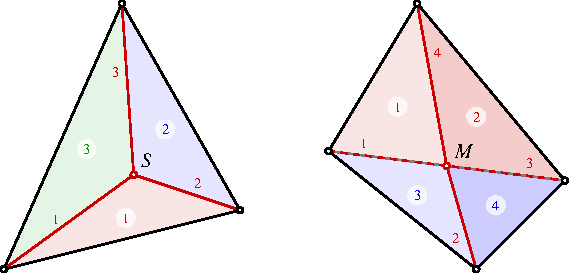
\includegraphics{chapters/120-topologie/images/unterteilung.pdf}
\caption{Links: Bei der Unterteilung eines einzelnen Dreiecks durch einen
inneren Punkt $S$ entstehen drei Dreieck ($+2$) und 3 neue Kanten.
Rechts: Bei der Unterteilung der Kante $AB$ durch den Punkt $M$ werden
\index{Unterteilung}%
beide Nachbardreiecke (rot und blau) in jeweils zwei Dreiecke ($+2)$ zerlegt.
Ausserdem entstehen drei zusätzliche Kanten.
\label{buch:topologie:eulercharakteristik:fig:unterteilung}}
\end{figure}
